\subsection{条件溯源流程实现}

条件溯源模块用于在投诉、恶意骚扰、虚假争议或平台审计场景下恢复必要身份信息。FoodShield 的条件溯源流程以订单号为入口，而不是以 PID 为入口。用户端和骑手端均可基于同一订单号提交溯源申请，管理员端统一处理申请并执行受控溯源。

溯源申请通常包含三个字段：\texttt{order\_id}、\texttt{reason} 和 \texttt{keyword}。其中，\texttt{order\_id} 用于确定目标订单，\texttt{reason} 用于说明溯源原因，\texttt{keyword} 用于指示需要检索的异常内容。系统要求溯源申请围绕订单发起，而不是允许管理员或普通用户任意输入 PID 进行身份查询。该设计更符合外卖平台实际纠纷处理流程，也降低了 PID 被滥用的风险。

管理员处理溯源申请时，系统首先执行完整性前置校验。服务器调用 Merkle 完整性验证模块，对目标订单的通信日志进行验证。若当前 Root 与历史快照 Root 不一致，系统认为该订单通信证据链可能已经被污染，拒绝继续执行溯源，并将失败原因写入审计日志。

若完整性验证通过，系统进一步根据申请中的关键词检索订单消息内容。由于数据库中保存的是 SM4-CBC 密文，服务器需要在内存中解密消息内容并执行关键词匹配。若未命中关键词，系统拒绝溯源并记录 \texttt{TRACE\_FAIL}；若命中关键词，系统根据命中消息的发送方 PID 查询 \texttt{users} 表，恢复必要的用户身份信息，并将结果返回给管理员端。

条件溯源流程可以抽象为：
\begin{figure}[H]
    \centering
    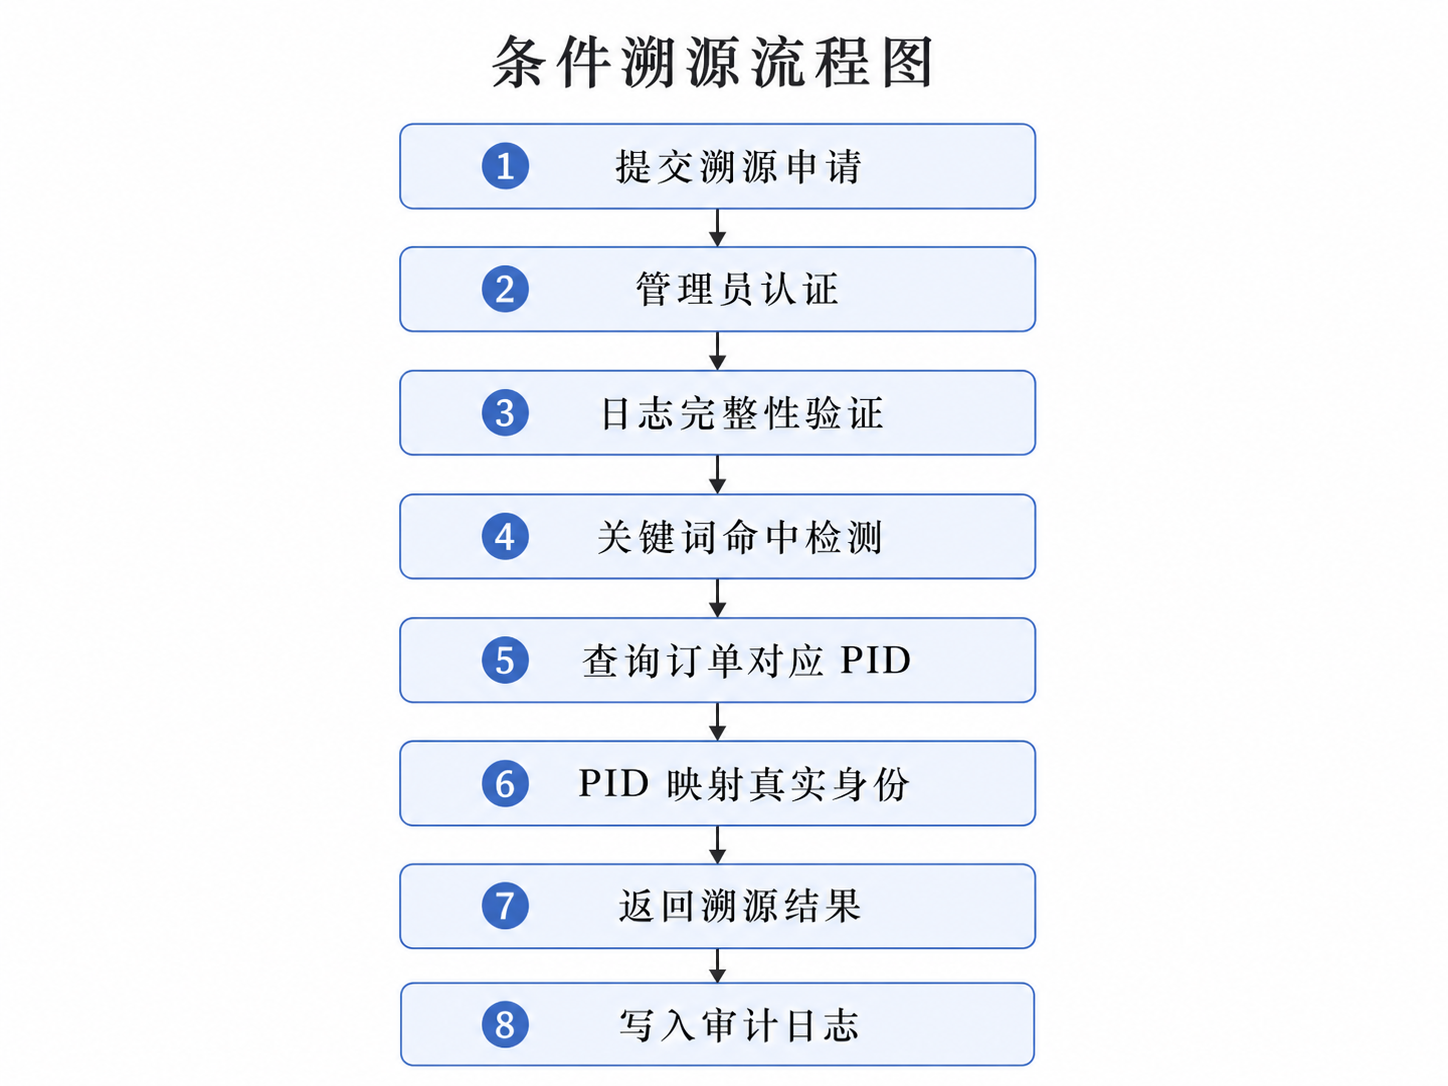
\includegraphics[width=0.95\textwidth]{content/chapter4/trace_flow.png}
    \caption{条件溯源流程图}
    \label{fig:trace-flow}
\end{figure}

\begin{figure}[H]
    \centering
    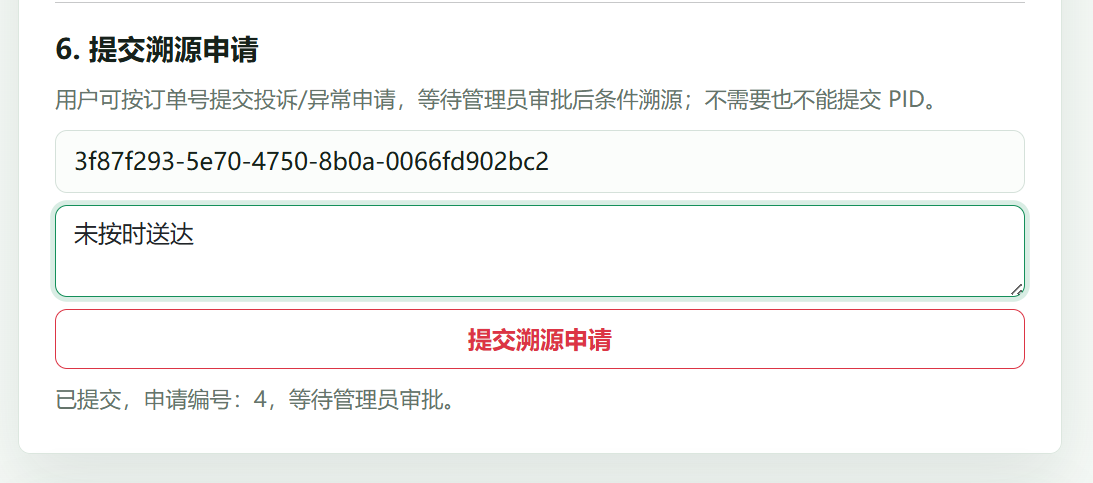
\includegraphics[width=0.9\textwidth]{content/chapter4/trace_request.png}
    \caption{订单溯源申请提交界面}
    \label{fig:trace-request}
\end{figure}

\begin{figure}[H]
    \centering
    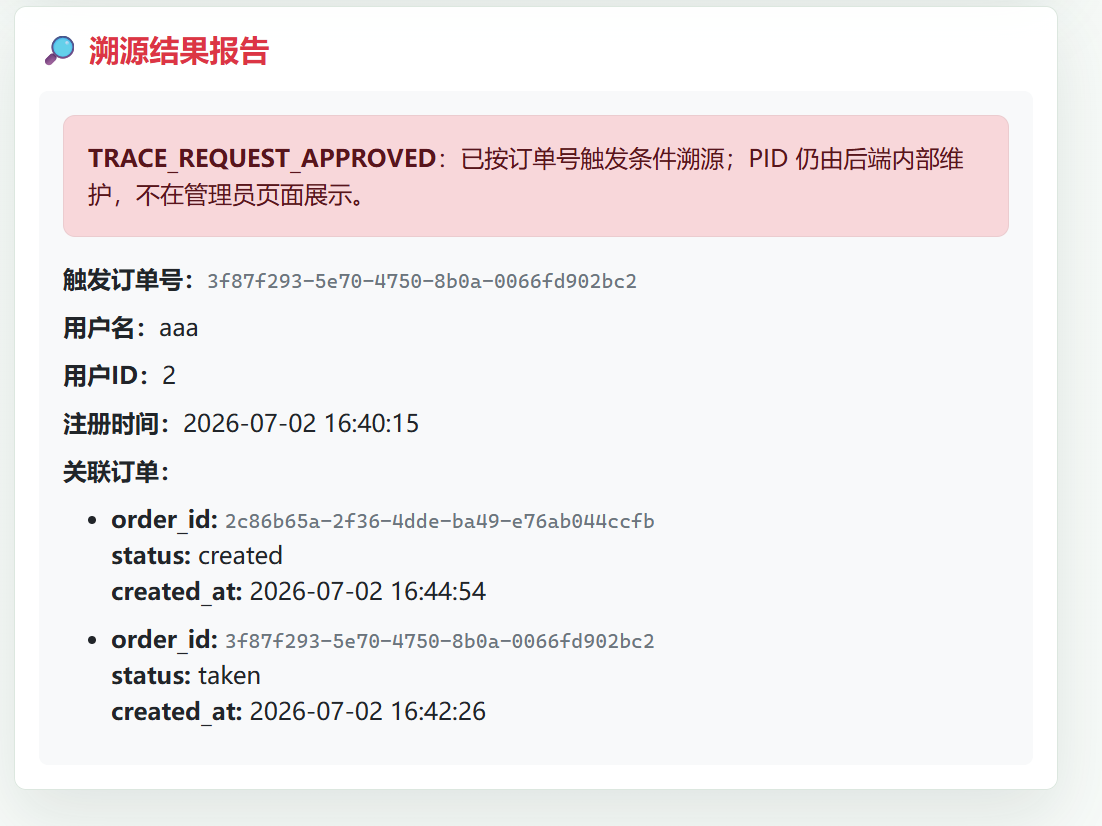
\includegraphics[width=0.95\textwidth]{content/chapter4/trace_success.png}
    \caption{条件溯源成功结果}
    \label{fig:trace-success}
\end{figure}

\begin{figure}[H]
    \centering
    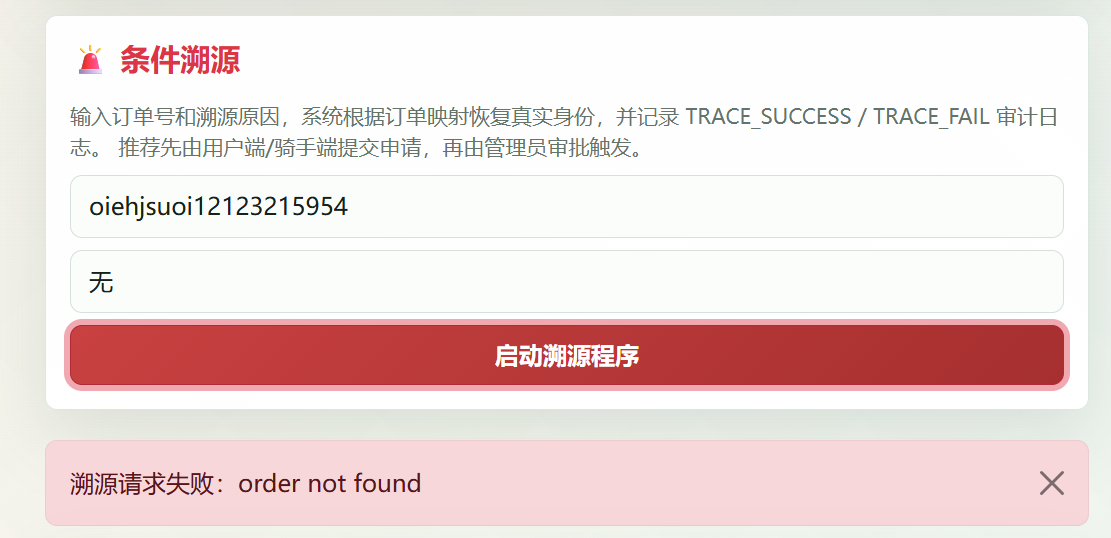
\includegraphics[width=0.95\textwidth]{content/chapter4/trace_fail.png}
    \caption{条件溯源失败结果}
    \label{fig:trace-fail}
\end{figure}

该流程体现了 FoodShield 的可控匿名思想：正常通信中不暴露真实身份，异常场景下也不能随意溯源，必须经过订单号入口、管理员认证、完整性验证和关键词命中等约束。这样既保留了平台管理能力，又降低了审计权限被滥用的风险。
